\subsection{So sánh hiệu năng truy xuất (Advanced RAG và Naive RAG)}

\textbf{Vai trò:}
Mô-đun truy xuất đóng vai trò quyết định trong việc thiết lập tập ngữ cảnh đầu vào cho mô hình sinh. Đánh giá này nhằm kiểm chứng sự vượt trội của kiến trúc RAG nâng cao (Advanced RAG) do đồ án đề xuất so với phương pháp RAG truyền thống (Naive RAG) trong việc định vị, bao phủ và ưu tiên các thông tin trọng yếu.

\textbf{Thiết lập so sánh:}
\begin{itemize}[leftmargin=*, label={}]
    \item \textbf{Naive RAG (Baseline):} Sử dụng chiến lược phân mảnh (\textit{chunking}) truyền thống, trong đó mỗi câu thoại được xem là một đơn vị ngữ nghĩa độc lập.
    \item \textbf{Advanced RAG (Hệ thống đề xuất):} Vận hành dựa trên quy trình tối ưu hóa đa tầng tích hợp các kỹ thuật: (i) Viết lại câu hỏi (\textit{Query Rewriting}) ở giai đoạn tiền truy xuất để làm rõ ngữ nghĩa dựa trên lịch sử hội thoại; (ii) Chiến lược \textit{Parent Document Retrieval} (băm nhỏ câu thoại thành các \textit{chunk} 40 từ với độ chồng lấp 10 từ) ở giai đoạn truy xuất để tăng mật độ vector; và (iii) Kết hợp bộ tái xếp hạng (\textit{Cross-Encoder}) cùng cơ chế Cửa sổ trượt (\textit{Sliding Window}) ở giai đoạn hậu truy xuất nhằm tinh lọc kết quả và khôi phục đầy đủ ngữ cảnh hội thoại.
\end{itemize}

\textbf{Tiêu chuẩn và Chỉ số đo lường:} 
Quá trình đánh giá tập trung vào khả năng tìm đúng tài liệu (\textbf{Hit Rate@K}), khả năng xếp hạng văn bản (\textbf{MRR}), và khả năng cô đọng thông tin (\textbf{Context Relevance}).

\textbf{Kết quả thực nghiệm:}
\begin{figure}[H]
    \centering
    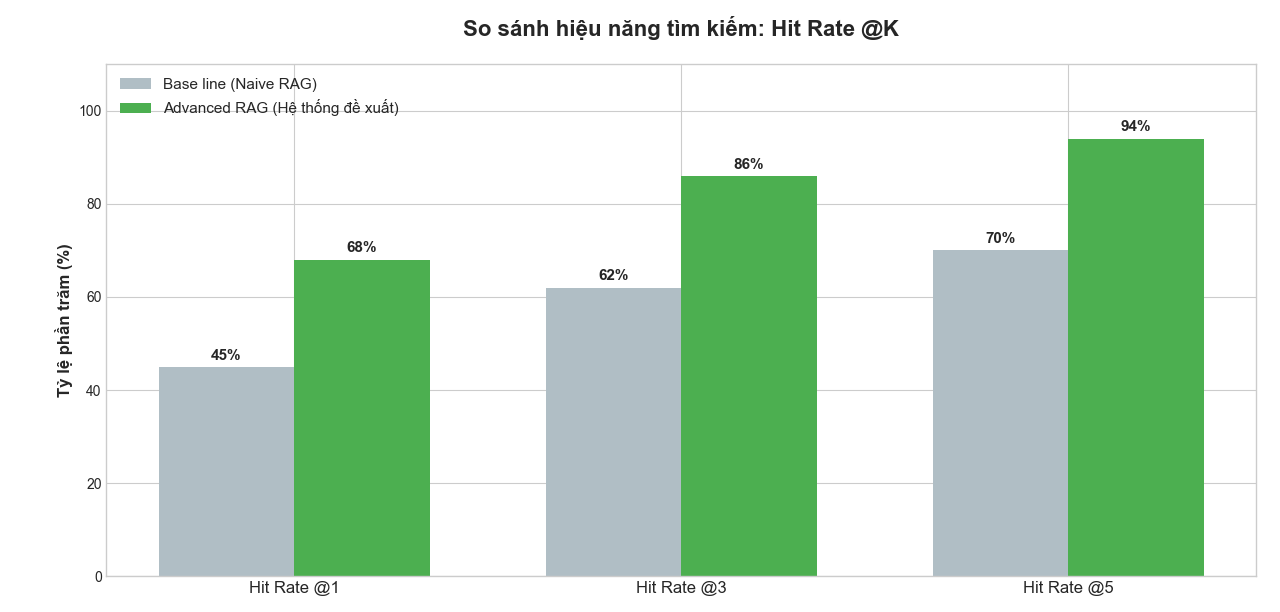
\includegraphics[width=1\textwidth]{images/danhgia1.png}
    \caption{So sánh hiệu năng truy xuất (Hit Rate @K) giữa phương pháp phân mảnh nguyên câu (Naive RAG) và hệ thống đề xuất với chiến lược Parent Document Retrieval (Advanced RAG)}
\end{figure}
Dựa trên tập dữ liệu đánh giá 50 truy vấn (Q\&A pairs), kiến trúc Advanced RAG cho thấy sự cải thiện toàn diện:
\begin{itemize}[leftmargin=*, label={}]
    \item \textbf{Về Hit Rate@K:} Hệ thống Advanced RAG đạt Hit Rate@1 là 68\% và Hit Rate@5 lên tới 94\%, cải thiện vượt bậc so với mức 45\% và 70\% của cấu hình Naive RAG.
    \item \textbf{Về MRR:} Điểm MRR của hệ thống đề xuất dao động dao động trong khoảng từ 0.756 đến 0.790, minh chứng cho việc các đoạn hội thoại chứa đáp án chính xác luôn được bộ tái xếp hạng ưu tiên đẩy lên các vị trí Top đầu.
    \item \textbf{Về Context Relevance:} Do hiệu ứng mở rộng của Cửa sổ trượt, điểm Context Relevance của Advanced RAG có sự sụt giảm nhẹ so với Naive RAG do hệ thống chủ động thu thập thêm các câu thoại lân cận.
\end{itemize}
\textbf{Nhận xét:}
Sự gia tăng đột phá của chỉ số Hit Rate khẳng định hiệu quả cộng hưởng từ chuỗi tối ưu hóa toàn diện của hệ thống Advanced RAG. Trong đó, việc viết lại câu truy vấn giúp xác định chính xác mục tiêu tìm kiếm, chiến lược \textit{Parent Document} giúp giải quyết triệt để điểm yếu cố hữu của Naive RAG là hiện tượng phân mảnh ngữ nghĩa (\textit{semantic fragmentation}). Đặc biệt, sự can thiệp của bộ tái xếp hạng (\textit{Cross-Encoder}) đóng vai trò quyết định trong việc sàng lọc nhiễu và đẩy các dẫn chứng thực sự liên quan lên vị trí ưu tiên, giúp tối ưu hóa chỉ số Hit Rate@1 và MRR. Mặc dù có sự đánh đổi nhỏ về Context Relevance do thu thập thêm một lượng hội thoại phụ trợ xung quanh, đây là sự hy sinh có chủ đích và tối ưu. Lượng thông tin mở rộng từ cơ chế cửa sổ trượt cung cấp đủ luồng giao tiếp (\textit{contextual flow}) làm cơ sở để Mô hình Ngôn ngữ Lớn (LLM) suy luận chính xác đối với các truy vấn phức tạp, loại bỏ hoàn toàn tình trạng đứt gãy thông tin khi chỉ truy xuất các câu thoại đơn lẻ.